\documentclass{article}
\usepackage{amsthm, amsmath, graphicx}
\usepackage[margin=1in]{geometry}
\begin{document}
    \noindent\textbf{CS 373 Homework 5}\hfill Anchu A. Lee\\
    \noindent\today\\\\
    \noindent\textbf{Question 1.10a} Construct NFA that recognizes the star of the language in Exercise 1.6b
        \begin{center}
            $\{w\mid w$ contains at least three 1s$\}$\\
            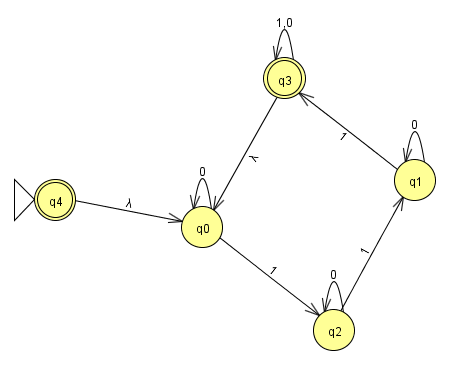
\includegraphics[scale=0.6]{q1}
        \end{center}
    \textbf{Question 1.10b} Same as before, but Exercise 1.6j
        \begin{center}
            $\{w\mid w $ contains at least two 0s and at most one 1$ \}$\\
            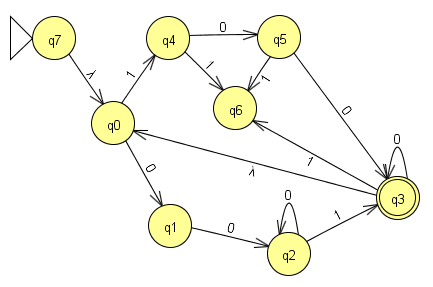
\includegraphics[scale=0.65]{q2}
        \end{center}
    \textbf{Question 1.29b} Use the pumping lemma to show that the language is not regular
        \begin{center}
            $A_2=\{www\mid w\in \{a,b\}^*\}$
        \end{center}
        \begin{proof}
            Assume $A_2$ is regular, then there must exist a number $n$ that is the pumping length. Test with the word $k = b^{n/2}b^{n/2}b^{n/2}$. $|k|>n$. Due to the nature of the language, there is only one way to split the word to satisfy the language. $x = b^{n/2}$; $y=b^{n/2}$; $z= b^{n/2}$. $|xy|\leq n$ and $|y|\geq 1$. Now consider pumping it up with $xy^iz$ for $i=2$. $xyz$ is not in $L$ because it is $b^{n/2}b^{n}b^{n/2}$ which does not match the definition of the language. Therefore our assumption was incorrect and $A_2$ is not regular.
        \end{proof}
    \textbf{Question 1.46a} Prove the following language is not regular using pumping lemma or closure of the class of regular languages under union, intersection, and compliment.
        \begin{center}
            $\{0^n1^m0^n\mid m,n \geq 0\}$
        \end{center}
        \begin{proof}
            Assume this language ($A$) is regular, so then there must exist a variable $p$, the pumping length. Choose $w = 0^p10^p$ as the test word. $|w|>p$ and $w\in A$. As $|xy|\leq p$, $x$ and $y$ must be composed of only zeros. Additionally, as $|y|>0$, $y$ would then have to equal $0^k$ for some $k>0$. For $xy^iz$, choose $i=0$ and the resulting word should still be in $A$. However $xy^0z=xz = 0^{p-k}10^p$. This resulting word is not in $A$ therefore our assumption was incorrect.
        \end{proof}
    \textbf{Question 1.46c} Same as before
        \begin{center}
            $\{w\mid w\in \{0,1\}^* $ is not a palindrome$ \}$
        \end{center}
        \begin{proof}
            Remember that $w$ is a palindrome if $w=w^R$. Assume that the language $L$ is regular. Then the compliment of $L$ should also be regular. $L' = \{w\mid w\in \{0,1\}^* $ is a palindrome$ \}$ is also regular. Now we can use the pumping lemma on $L'$. \\
            There exists a $p$ by the pumping lemma. Choose the word $0^p10^p$. $|w|\geq p$. Because $|xy|\leq p$, $x$, $y$ must be composed of only zeros. Additionally as $|y|>0$, $y$ would have to equal $0^k$ for some $k>0$. Finally take $xy^iz$ for $i=0$. Then the resulting word would equal $0^{p-k}10^p$ which cannot be a palindrome since $p-k<p$. This contradicts the assumptiong that $L$ is regular.
        \end{proof}
    \textbf{Question 1.46d} Same as before
        \begin{center}
            $\{wtw \mid w,t \in \{0.1\}^+ \}$
        \end{center}
        \begin{proof}
            Assume the language ($L$) is regular. Then by the pumping lemma, there exists a $p$. Choose the word $d=0^p110^p1$. $|d|\geq p$. To comply with the conditions for pumping lemma, $x$ and $y$ must both consist of only zeros as $|xy|\leq p$. That means $y=0^k$ for some $k>0$. Next, for some $i$, $xy^iz\in L$. Set $i=2$ and the resulting word is $0^{p+k}110^p1$. As $p+k > p$ this word cannot be in the language $L$ and therefore the assumption that $L$ is regular is false.  
        \end{proof}
    \textbf{Question 1.47} Let $\sum = \{1,\#\}$ and let 
        \begin{center}
            $Y=\{w\mid w=x_1\#x_2\#...\#x_k $ for $ k \geq 0 $, each $ x_i\in 1^* $, and $ x_i\not= x_j $ for $ i\not= j \}$
        \end{center}
        Prove $Y$ is not regular.
        \begin{proof}
            Assume the language $Y$ is regular. Then let $p$ be the pumping length from the pumping lemma. Consider the word $w=1^p\#1^{p+1}\#...\#1^{2p}$. $|xy|\leq p$ so $x$ and $y$ must compose of only $1$s. Then $y=1^k$ for some $k>0$. Now consider $t = xy^iz$ for $i=2$. $t$ can also be written out as $t=t_0\#t_1\#...\#t_u$ where $u=p$, $t_0=1^{p+|y|}$ and for $1\leq j \leq p$, $t_j=1^{p+j}$. Since $1\leq |y|\leq p$, we can find that $p+1\leq (p+|y|) \leq 2p$ and then $t_0=t_{p+|y|}$. Two series of 1s are equal to each other and therefore $t$ cannot be in the language $Y$. This contradicts our assumption that $Y$ was regular.
        \end{proof}
    \noindent\textbf{Question 1.49}
        \begin{itemize}
            \item Let $B= \{1^ky\mid y\in \{0,1\}^*$ and $y$ contains at least $k$ 1s, for $k\geq 1\}$.\\
                  Show that $B$ is a regular language.
                  \begin{proof}
                      If $B$ is a regular language, then it can be expressed by a regular expression. Set $k=2$ $110^*10^*1(0\cup 1)^*$. This language is regular.
                  \end{proof}
            \item Let $C= \{1^k y\mid y\in \{0,1\}^* $ and $y$ contains at most $k$ 1s, for $k\geq 1\}$.\\
                  Show that $C$ isn't a regular language.
                  \begin{proof}
                      Assume that $C$ is a regular language, then let $p$ be the pumping length from the pumping lemma. Consider the word $s=1^p0^p1^p$. As $|xy|\leq p$, $x$ and $y$ must both only consist of 1s. Then $y=1^t$ for some $t>0$. Now consider $xy^iz$ for $i=0$ which would look like $1^{p-t}0^p1^p$. As $p-t<p$ the word is not in $C$ and violates the assumption that $C$ is a regular language.
                  \end{proof}
        \end{itemize}
    \textbf{Show that $\{0^n1^m2^k\mid k$ divides $n+m\}$ is not regular.}\\
    \textbf{Convert the following NFA to a DFA}:\\
    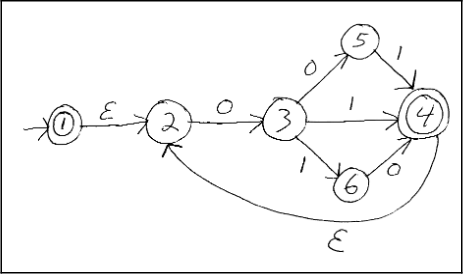
\includegraphics[scale=0.75]{machine}
\end{document}